% Graphic for TeX using PGF
% Title: /home/martin/repositories/TDDD77/dokumentation/kandidatrapport/martin-tex/Diagram1.dia
% Creator: Dia v0.97.2
% CreationDate: Thu Apr 16 11:23:03 2015
% For: martin
% \usepackage{tikz}
% The following commands are not supported in PSTricks at present
% We define them conditionally, so when they are implemented,
% this pgf file will use them.
\ifx\du\undefined
  \newlength{\du}
\fi
\setlength{\du}{15\unitlength}
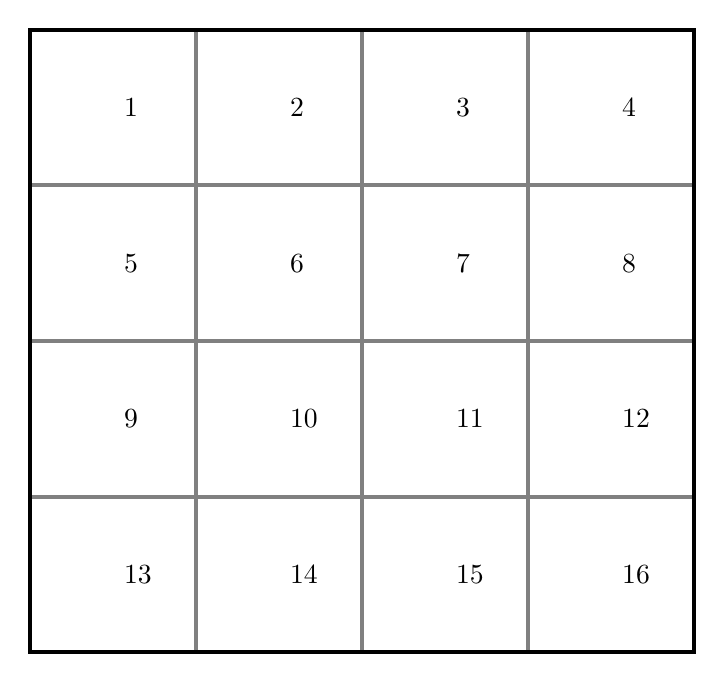
\begin{tikzpicture}
\pgftransformxscale{1.000000}
\pgftransformyscale{-1.000000}
\definecolor{dialinecolor}{rgb}{0.000000, 0.000000, 0.000000}
\pgfsetstrokecolor{dialinecolor}
\definecolor{dialinecolor}{rgb}{1.000000, 1.000000, 1.000000}
\pgfsetfillcolor{dialinecolor}
\pgfsetmiterjoin
\pgfsetdash{}{0pt}
\definecolor{dialinecolor}{rgb}{1.000000, 1.000000, 1.000000}
\pgfsetfillcolor{dialinecolor}
\fill (0.044745\du,1.818031\du)--(0.044745\du,16.818031\du)--(16.044745\du,16.818031\du)--(16.044745\du,1.818031\du)--cycle;
\pgfsetlinewidth{0.100000\du}
\definecolor{dialinecolor}{rgb}{0.500000, 0.500000, 0.500000}
\pgfsetstrokecolor{dialinecolor}
\draw (0.044745\du,5.568031\du)--(16.044745\du,5.568031\du);
\definecolor{dialinecolor}{rgb}{0.500000, 0.500000, 0.500000}
\pgfsetstrokecolor{dialinecolor}
\draw (0.044745\du,9.318031\du)--(16.044745\du,9.318031\du);
\definecolor{dialinecolor}{rgb}{0.500000, 0.500000, 0.500000}
\pgfsetstrokecolor{dialinecolor}
\draw (0.044745\du,13.068031\du)--(16.044745\du,13.068031\du);
\definecolor{dialinecolor}{rgb}{0.500000, 0.500000, 0.500000}
\pgfsetstrokecolor{dialinecolor}
\draw (4.044745\du,1.818031\du)--(4.044745\du,16.818031\du);
\definecolor{dialinecolor}{rgb}{0.500000, 0.500000, 0.500000}
\pgfsetstrokecolor{dialinecolor}
\draw (8.044745\du,1.818031\du)--(8.044745\du,16.818031\du);
\definecolor{dialinecolor}{rgb}{0.500000, 0.500000, 0.500000}
\pgfsetstrokecolor{dialinecolor}
\draw (12.044745\du,1.818031\du)--(12.044745\du,16.818031\du);
\pgfsetlinewidth{0.100000\du}
\definecolor{dialinecolor}{rgb}{0.000000, 0.000000, 0.000000}
\pgfsetstrokecolor{dialinecolor}
\draw (0.044745\du,1.818031\du)--(0.044745\du,16.818031\du)--(16.044745\du,16.818031\du)--(16.044745\du,1.818031\du)--cycle;
% setfont left to latex
\definecolor{dialinecolor}{rgb}{0.000000, 0.000000, 0.000000}
\pgfsetstrokecolor{dialinecolor}
\node[anchor=west] at (8.044745\du,9.318031\du){};
% setfont left to latex
\definecolor{dialinecolor}{rgb}{0.000000, 0.000000, 0.000000}
\pgfsetstrokecolor{dialinecolor}
\node[anchor=west] at (4.000000\du,8.000000\du){};
% setfont left to latex
\definecolor{dialinecolor}{rgb}{0.000000, 0.000000, 0.000000}
\pgfsetstrokecolor{dialinecolor}
\node[anchor=west] at (8.044745\du,9.318031\du){};
% setfont left to latex
\definecolor{dialinecolor}{rgb}{0.000000, 0.000000, 0.000000}
\pgfsetstrokecolor{dialinecolor}
\node[anchor=west] at (4.900000\du,6.700000\du){};
% setfont left to latex
\definecolor{dialinecolor}{rgb}{0.000000, 0.000000, 0.000000}
\pgfsetstrokecolor{dialinecolor}
\node[anchor=west] at (2.044745\du,3.693031\du){1};
% setfont left to latex
\definecolor{dialinecolor}{rgb}{0.000000, 0.000000, 0.000000}
\pgfsetstrokecolor{dialinecolor}
\node[anchor=west] at (6.044745\du,3.693031\du){2};
% setfont left to latex
\definecolor{dialinecolor}{rgb}{0.000000, 0.000000, 0.000000}
\pgfsetstrokecolor{dialinecolor}
\node[anchor=west] at (10.044745\du,3.693031\du){3};
% setfont left to latex
\definecolor{dialinecolor}{rgb}{0.000000, 0.000000, 0.000000}
\pgfsetstrokecolor{dialinecolor}
\node[anchor=west] at (14.044745\du,3.693031\du){4};
% setfont left to latex
\definecolor{dialinecolor}{rgb}{0.000000, 0.000000, 0.000000}
\pgfsetstrokecolor{dialinecolor}
\node[anchor=west] at (2.044745\du,7.443031\du){5};
% setfont left to latex
\definecolor{dialinecolor}{rgb}{0.000000, 0.000000, 0.000000}
\pgfsetstrokecolor{dialinecolor}
\node[anchor=west] at (6.044745\du,7.443031\du){6};
% setfont left to latex
\definecolor{dialinecolor}{rgb}{0.000000, 0.000000, 0.000000}
\pgfsetstrokecolor{dialinecolor}
\node[anchor=west] at (10.044745\du,7.443031\du){7};
% setfont left to latex
\definecolor{dialinecolor}{rgb}{0.000000, 0.000000, 0.000000}
\pgfsetstrokecolor{dialinecolor}
\node[anchor=west] at (14.044745\du,7.443031\du){8};
% setfont left to latex
\definecolor{dialinecolor}{rgb}{0.000000, 0.000000, 0.000000}
\pgfsetstrokecolor{dialinecolor}
\node[anchor=west] at (2.044745\du,11.193031\du){9};
% setfont left to latex
\definecolor{dialinecolor}{rgb}{0.000000, 0.000000, 0.000000}
\pgfsetstrokecolor{dialinecolor}
\node[anchor=west] at (6.044745\du,11.193031\du){10};
% setfont left to latex
\definecolor{dialinecolor}{rgb}{0.000000, 0.000000, 0.000000}
\pgfsetstrokecolor{dialinecolor}
\node[anchor=west] at (10.044745\du,11.193031\du){11};
% setfont left to latex
\definecolor{dialinecolor}{rgb}{0.000000, 0.000000, 0.000000}
\pgfsetstrokecolor{dialinecolor}
\node[anchor=west] at (14.044745\du,11.193031\du){12};
% setfont left to latex
\definecolor{dialinecolor}{rgb}{0.000000, 0.000000, 0.000000}
\pgfsetstrokecolor{dialinecolor}
\node[anchor=west] at (2.044745\du,14.943031\du){13};
% setfont left to latex
\definecolor{dialinecolor}{rgb}{0.000000, 0.000000, 0.000000}
\pgfsetstrokecolor{dialinecolor}
\node[anchor=west] at (6.044745\du,14.943031\du){14};
% setfont left to latex
\definecolor{dialinecolor}{rgb}{0.000000, 0.000000, 0.000000}
\pgfsetstrokecolor{dialinecolor}
\node[anchor=west] at (10.044745\du,14.943031\du){15};
% setfont left to latex
\definecolor{dialinecolor}{rgb}{0.000000, 0.000000, 0.000000}
\pgfsetstrokecolor{dialinecolor}
\node[anchor=west] at (14.044745\du,14.943031\du){16};
\end{tikzpicture}
